\begin{figure}
    \centering
    %\vspace{-1em}
    \begin{subfigure}[b]{0.6\linewidth} % 40% width
        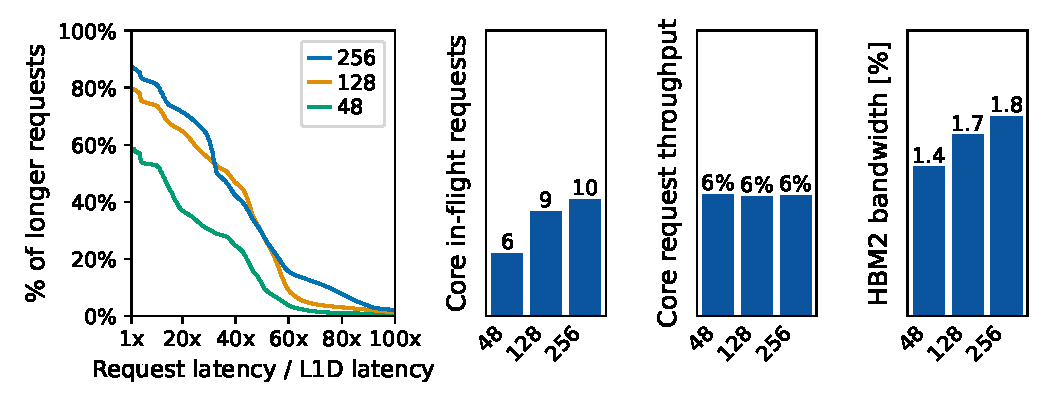
\includegraphics[width=\linewidth]{img_embedding_implications_arxiv.pdf}
        \vspace{-2em}
        \caption{\texttt{arxiv} statistics}
        %\vspace{0.5em}
        \label{fig:ltu-arxiv}
    \end{subfigure}
    \begin{subfigure}[b]{0.6\linewidth} % 40% width
        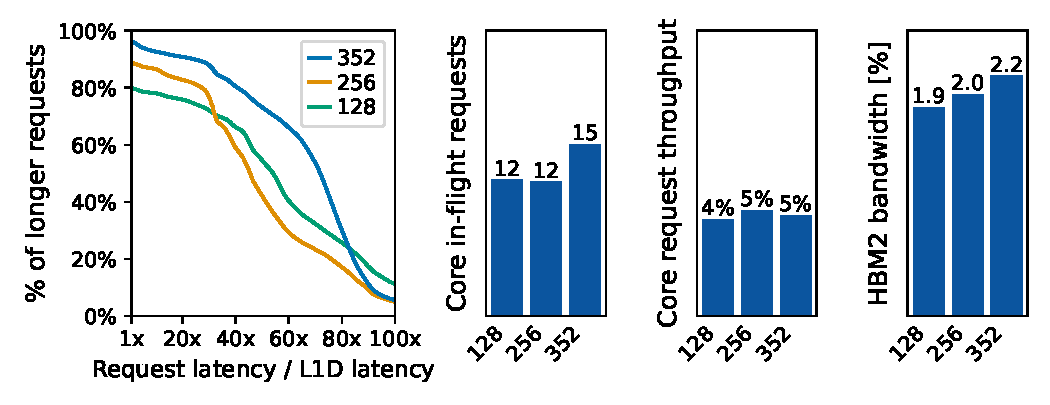
\includegraphics[width=\linewidth]{img_embedding_implications_mag.pdf}
        \vspace{-2em}
        \caption{\texttt{mag} statistics}
        %\vspace{0.5em}
        \label{fig:ltu-mag}
    \end{subfigure}
    \begin{subfigure}[b]{0.6\linewidth} % 40% width
        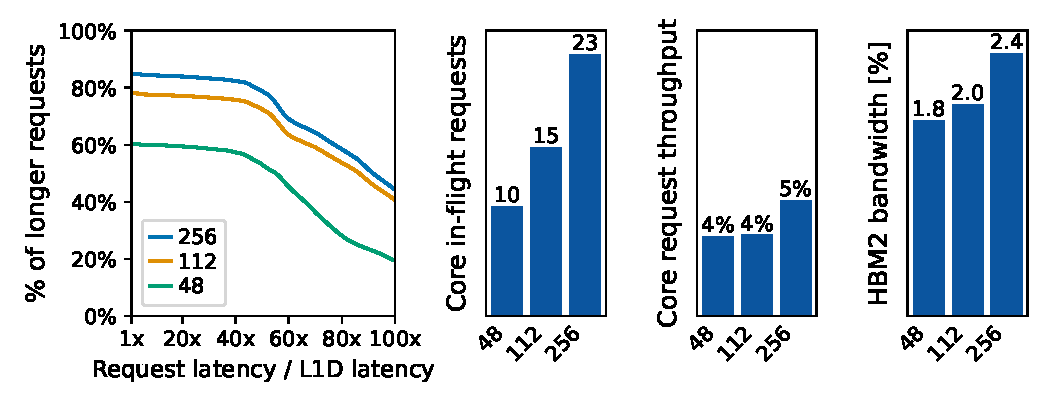
\includegraphics[width=\linewidth]{img_embedding_implications_products.pdf}
        \vspace{-2em}
        \caption{\texttt{products} statistics}
        %\vspace{0.5em}
        \label{fig:ltu-products}
    \end{subfigure}
    \begin{subfigure}[b]{0.6\linewidth} % 40% width
        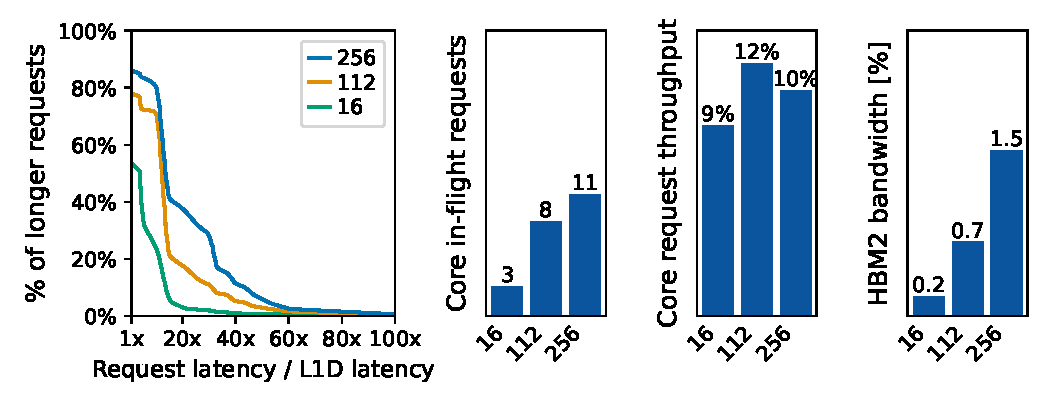
\includegraphics[width=\linewidth]{img_embedding_implications_proteins.pdf}
        \vspace{-2em}
        \caption{\texttt{proteins} statistics}
        %\vspace{0.5em}
        \label{fig:ltu-proteins}
    \end{subfigure}
    %\vspace{-2em}
    \caption[Architectural implications of long embedding lookups on an off-the-shelf CPU core.]{Architectural implications of long embedding lookups on an off-the-shelf CPU core. Rows correspond to different datasets, whereas lines and bars correspond to different embedding sizes. The first column shows that a large fraction of embedding lookups in GNN models take orders of magnitude longer than L1D accesses. For \texttt{products}---the dataset with the lowest locality---more than 74\% of memory requests (y-axis) are 10$\times$ longer than an L1D access (x-axis), and 40\% are more than 100$\times$ longer, as they need to reach HBM. As shown in the second column, the higher the average latency, the higher the number of in-flight requests tracked by the core. However, CPU cores can only track a few requests before the whole pipeline stalls. As shown in the third column, due to these stalls, the core issues memory requests at a fraction of its peak throughput of one request per cycle. Even \texttt{proteins}---the dataset with the highest locality---only achieves up to 12\% throughput. As shown in the fourth column, this results in low HBM per-core utilization. Even a low-locality dataset like \texttt{products}---with the majority of accesses reaching HBM---utilizes up to 2.4\% bandwidth.}
    \label{fig:embedding-implications-combined}
\end{figure}
